\section{Sintesi e caratterizzazione con 1H NMR di \ce{HCo[P(OPh)3]4}}
\subsection{Sintesi}
\subsubsection{Procedura sperimentale}
Abbiamo sciolto $0.5 \mathrm{~g}$ di nitrato di cobalto (II) esaidrato in $10 \mathrm{~mL}$ di etanolo e abbiamo aggiunto tramite pipetta graduata $2.5 \mathrm{~g}$ (circa $2.1 \mathrm{~mL}$) di trifenilfosfito. Abbiamo preparato a parte una soluzione di $0.20 \mathrm{~g}$ di sodio boroidruro in $5.0 \mathrm{~mL}$ di etanolo e quindi aggiunto goccia a goccia quest'ultima soluzione alla precedente su un intervallo di oltre mezz'ora. Il colore della soluzione vira dal rosso al giallo. Quindi filtriamo su Buchner e laviamo con etanolo, acqua e metanolo. Ridissolviamo il precipitato in $15 \mathrm{~mL}$ di diclorometano e poi con difficoltà filtriamo su Buchner per eliminare le impurità indissolte. Infine, riprecipitiamo con etanolo e raccolgliamo il complesso idrurico filtrando su Buchner.
\subsubsection{Commenti e osservazioni}

Durante l'aggiunta potevamo notare che nell'intorno del punto di contatto tra la goccia di sodioboroidruro e la soluzione si formava una zona bruna. Questo può essere causato dalla formazione di particelle di cobalto\cite{cored}.
Le dimensioni delle particelle di cobalto prodotte dipendono sensibilmente da una molteplicità di fattori diversi, questo spiega anche il fatto che per ogni gruppo le miscele avevano colori variabili. Nella zona dove avveniva l'immissione della soluzione 
 la concentrazione di \ce{NaBH4} era elevata e le particelle prodotte avevano dimensioni mesoscopiche dando alla soluzione un colore bruno. Nelle zone dove il sodioboroidruro era presente in minor quantità la dimensione delle particelle era minore, questo poteva produrre effetti di cambio di colore. Infatti, il colore di una sospensione di nanoparticelle di un metallo dipende dalle dimensioni di quest'ultime. 
La soluzione di etanolo dopo la notte aveva preso una colorazione sul verde acqua. Probabilmente questo è dovuto al fatto che il filtro non era stato lavato correttamente e parte dell'acido cloridrico usato dal gruppo precedente per la pulizia era rimasto nei pori e aveva trasformato parte dell'idruro in cloruro.
\subsubsection{Calcoli e analisi dei dati}



In partenza avevamo un numero di moli di reagenti pari a
\[ n_{\ce{Co(NO3)2.6H2O}}=\frac{0.5 \mathrm{~g}}{291.03 \mathrm{~g} / \mathrm{mol}}= 1.72 \mathrm{~mmol} \]

\[ n_{\ce{P(OPh)3}}=\frac{2.1 \mathrm{~mL} \cdot 1.184 \mathrm{~g} / \mathrm{mL} }{310.28 \mathrm{~g} / \mathrm{mol}}= 8.057 \mathrm{~mmol} \]

\[ n_{\ce{NaBH4}}=\frac{0.2 \mathrm{~g}  }{37.83 \mathrm{~g} / \mathrm{mol}}= 5.287 \mathrm{~mmol} \]

Considerando quindi la stechiometria $1: 3: 1$ notiamo che il sale di cobalto è il reagente limitante. 



Calcoliamo la resa 
\[ Y_\% = \frac{n_\text{pro}}{n_{\ce{Co(NO3)2.6H2O}}}\cdot 100 \]

Le moli finali sono il rapporto massa della provettà piena di prodotto tolta la tara e la massa molare del prodotto.

\[ n_\text{pro} = \frac{(m_{f} - m_{t})}{M_\text{pro}} 
 = \frac{ 15.6794 \um{g} - 15.0190 \um{g} }{ 1301.02 \um{g/mol}} =  \frac{0.6604 \mathrm{~g}}{1301.02 \mathrm{~g} / \mathrm{mol}}=0.508 \um{mmol}\]

\[ Y_\% = \frac{n_\text{pro}}{n_{\ce{HCo(OPh)3}}}\cdot 100  = \frac{  0.508 \cdot 10^{-3} \mathrm{~mol}}{1.72 \cdot 10^{-3} \mathrm{~mol}} \cdot 100 =29.5\%\]

\subsection{Spettro NMR}


\begin{figure}
    \centering
    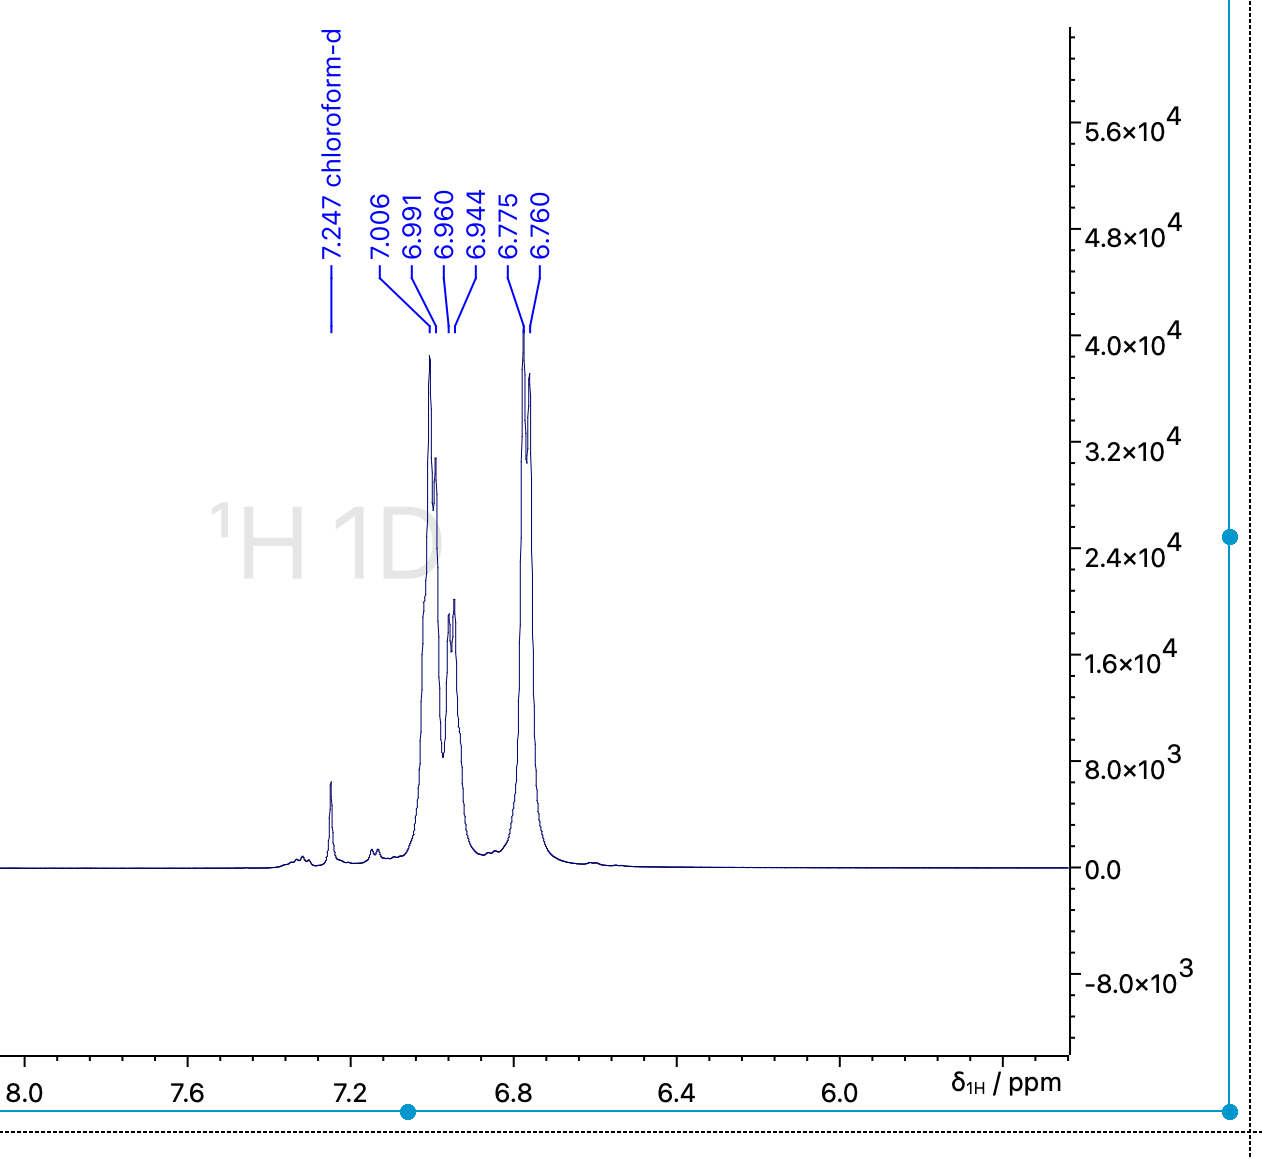
\includegraphics[width=0.8\linewidth]{Relazione/foto/CoH_aromaticpeak_calc_zoom.png}
    \caption{Caption}
    \label{fig:coharomaticzoom}
\end{figure}

\begin{figure}
    \centering
    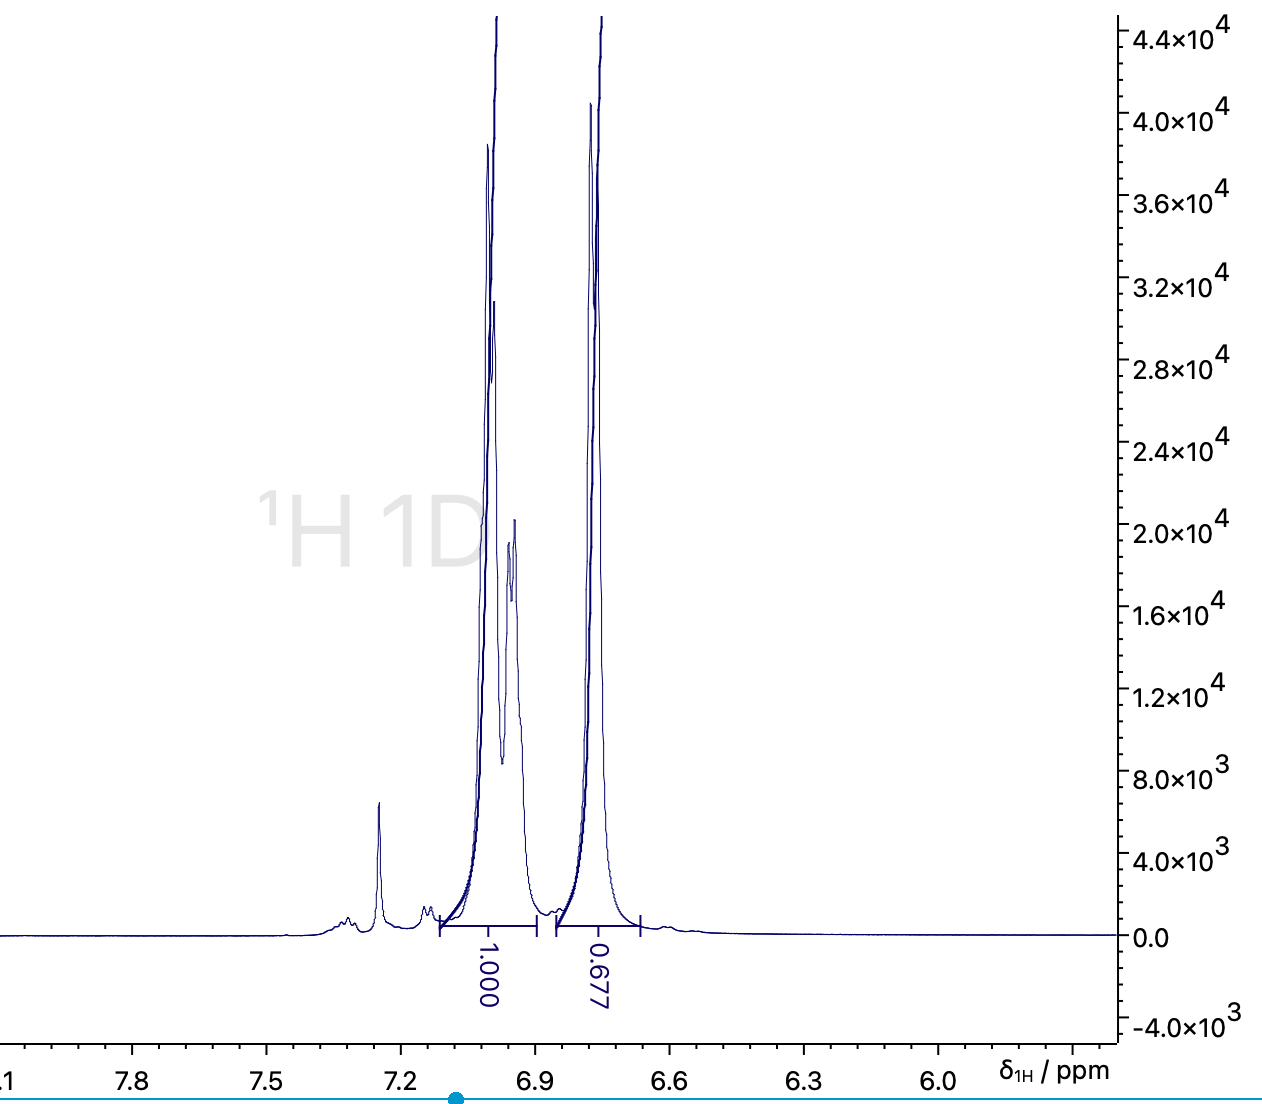
\includegraphics[width=0.8\linewidth]{Relazione/foto/CoH_aromaticpeak_right.png}
    \caption{Caption}
    \label{fig:my_label}
\end{figure}


\begin{figure}
    \centering
    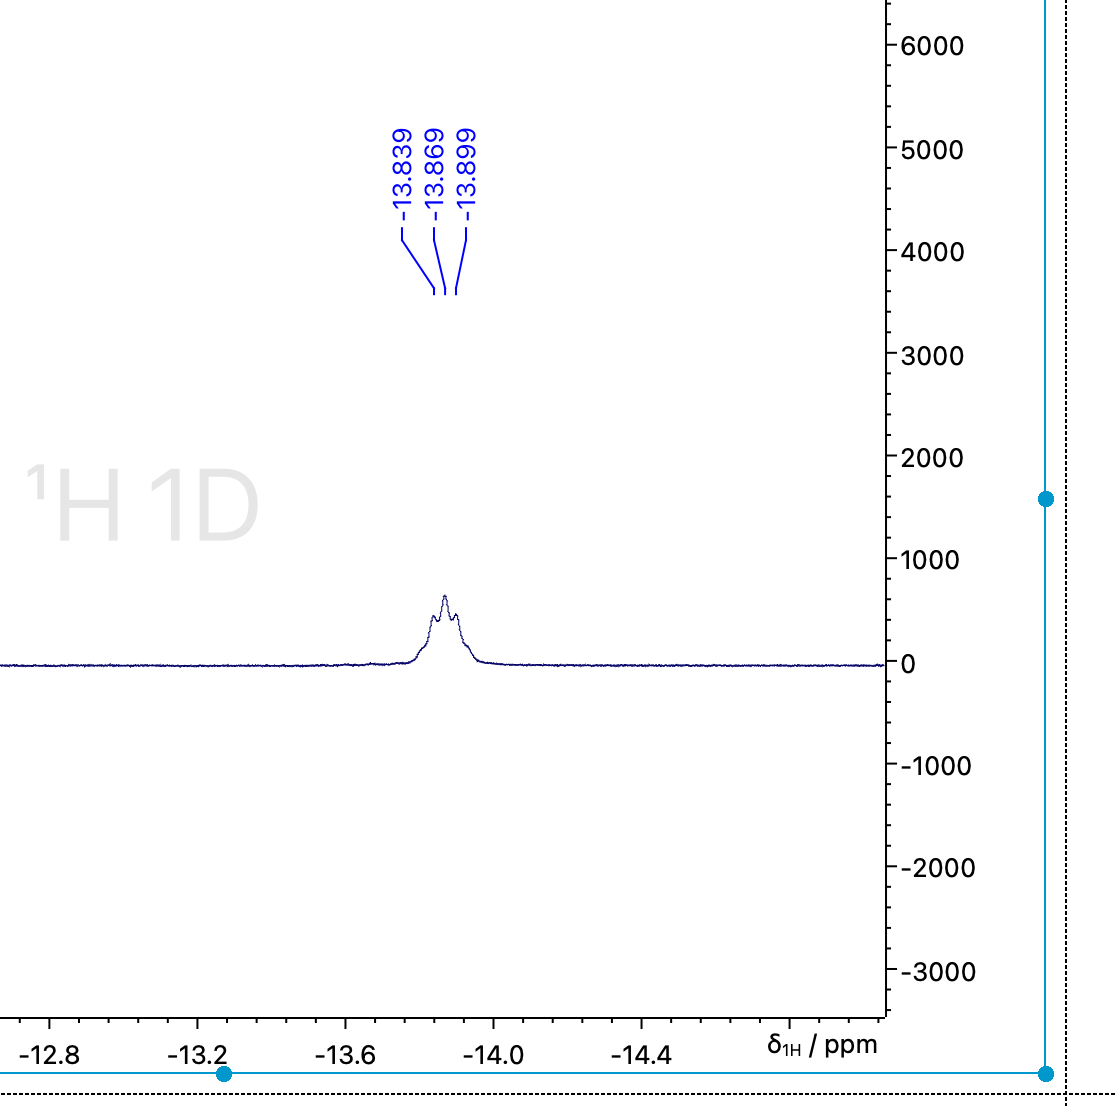
\includegraphics[width=0.8\linewidth]{Relazione/foto/CoH_hydridepeak_calc.png}
    \caption{Caption}
    \label{fig:my_label}
\end{figure}
\begin{figure}
    \centering
    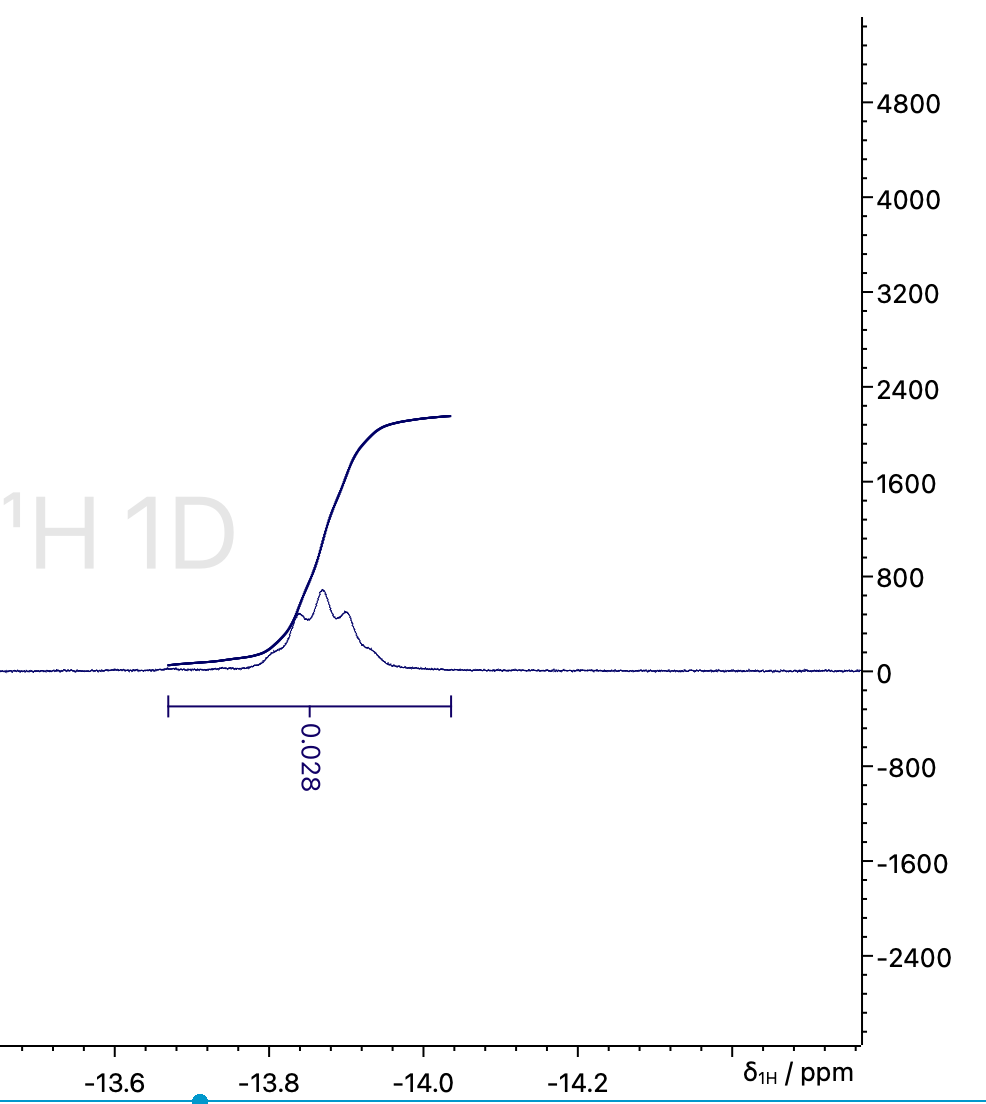
\includegraphics[width=0.8\linewidth]{Relazione/foto/CoH_hydridepeak_right.png}
    \caption{Caption}
    \label{fig:my_label}
\end{figure}



